% Figure block for the locked R-Universe finite-window theory.
% Filenames intentionally match files in the Overleaf project root.

\begin{figure}[htbp]
\centering
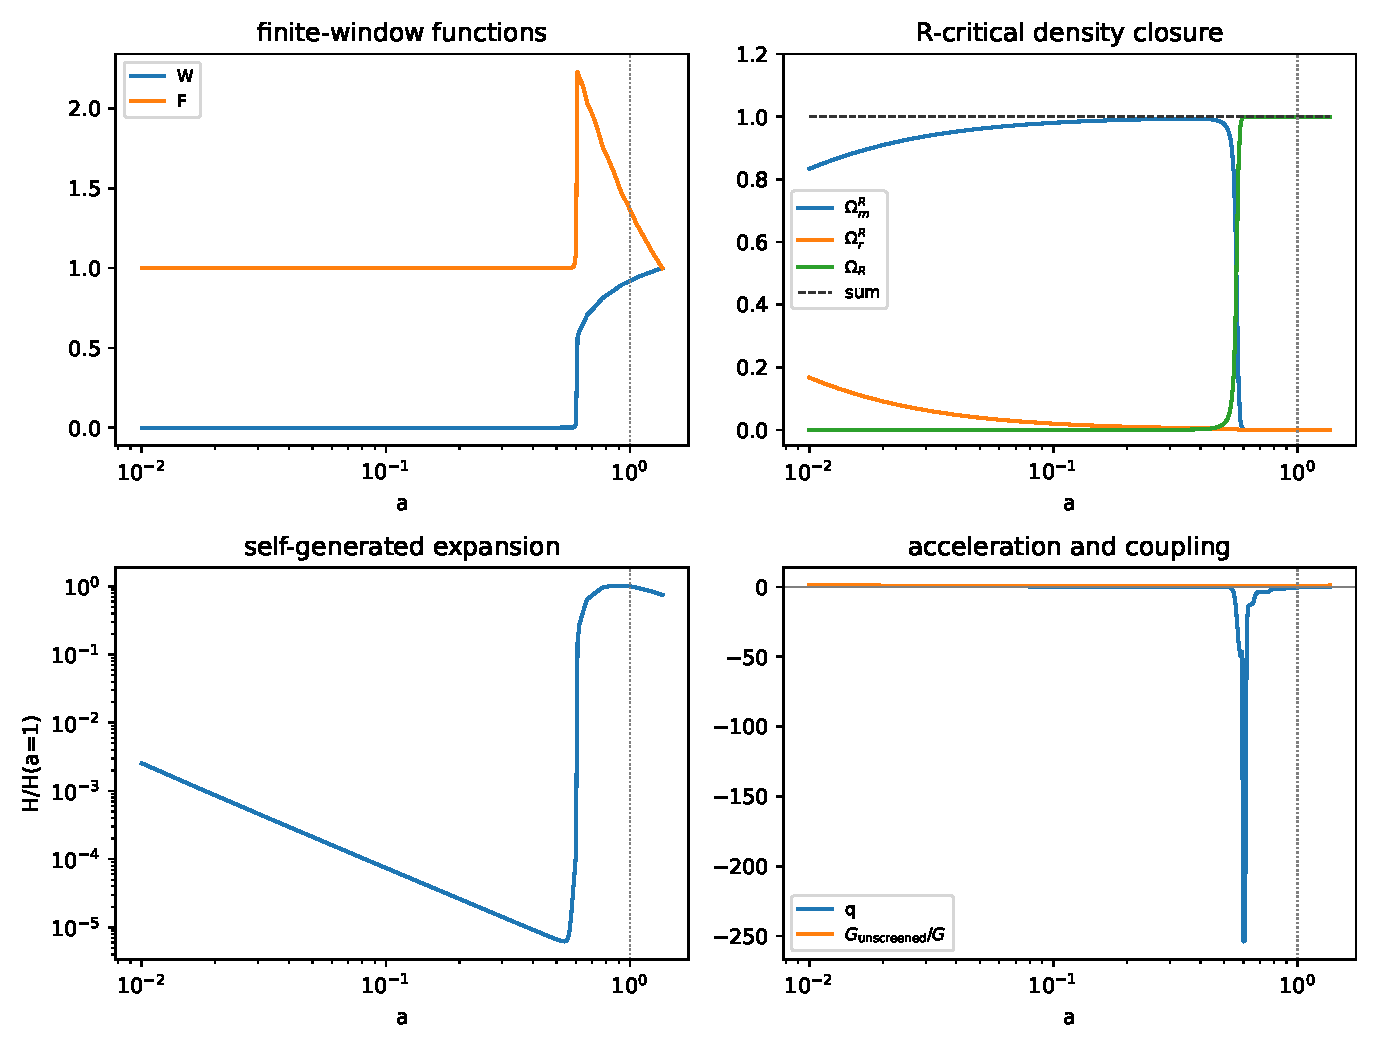
\includegraphics[draft=false,width=0.98\linewidth]{figures/fig01_locked_r_universe_background.pdf}
\caption{Reduced-branch background integration of the locked trace-scalar finite-window equations. The branch is self-accelerating in the reduced subsystem, but it is not a physical solution of the full multiplier action because the multiplier stress tensor, the independent multiplier equation and the matter-variation terms induced by $\lambda T$ have been omitted. It is retained only as a diagnostic showing why the reduced system cannot be used as the final theory.}
\label{fig:locked-background}
\end{figure}

\begin{figure}[htbp]
\centering
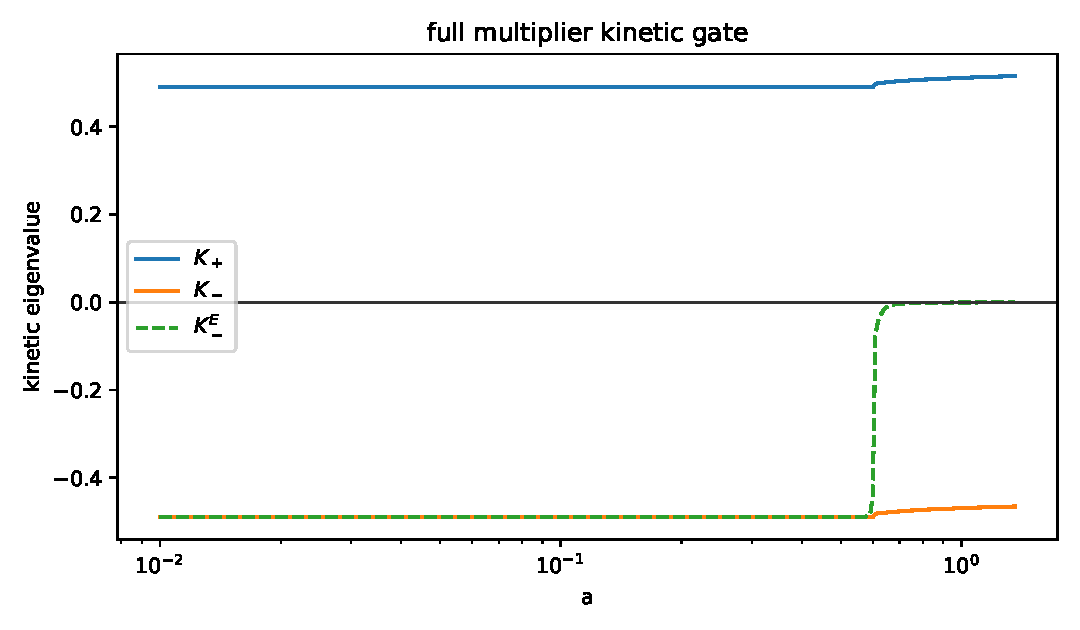
\includegraphics[draft=false,width=0.82\linewidth]{figures/fig02_full_lambda_ghost_gate.pdf}
\caption{Full multiplier kinetic gate. After integrating the multiplier term by parts, the Jordan-frame scalar velocity Hessian in $(\dot R_c,\dot\lambda)$ is $K=\begin{pmatrix}Z&\ell^2\\ \ell^2&0\end{pmatrix}$. Its determinant is $-\ell^4$, so for every finite nonzero $\ell$ one eigenvalue is negative. Including the positive Einstein-frame contribution to the $R_cR_c$ entry leaves $\det K_E=-\ell^4/F^2<0$. The plotted branch confirms the negative mode over the integrated background.}
\label{fig:lambda-ghost-gate}
\end{figure}
